\documentclass{jarticle} %LaTeX2e


\usepackage{color}
%\usepackage{graphicx}
\usepackage[dvipdfmx]{graphicx} % pdfを使用する
\usepackage{tabularx}
\usepackage{fancyhdr} % header, footer
\usepackage{lastpage} % 総page数
\usepackage{multirow}
\usepackage{ulem}
\usepackage{latexsym}
\usepackage{maltcol}
\usepackage{jumoline}
\usepackage{caption}
\usepackage{url}

\setlength{\UnderlineTexDepth}{3pt}

\newcommand{\todo}[1]{\colorbox{yellow}{{\bf TODO}:}{\color{blue}{\textbf{[#1]}}}}

\newcommand{\ihara}[1]{\colorbox{green}{{\bf ihara}:}{\color{red}{\textbf{[#1]}}}}

\renewcommand{\headrulewidth}{0pt} % ヘッダーラインを打ち出さない

% todayコマンド 西暦表示
\renewcommand{\today}{%
  \the\year /%
   {\ifnum \month < 10  0\the\month \else \the\month \fi}/%
   {\ifnum \day < 10  0\the\day \else \the\day \fi}%
}

% header, footer周りの定義
\pagestyle{fancy}

% 回答文タイトル
\def\restitle{条件付論文に対する回答文}
\def\paptitle{Scratchユーザのコンピュテーショナル・シンキングスキルの\\習熟過程の共通性分析と習熟度到達予測}

%% header
\lhead{\restitle}
\rhead{\paptitle}

%% footer
\cfoot{}
\lfoot{\date{\today}}
\lfoot{\today}
\rfoot{\thepage/\pageref{LastPage}}

%% ページの余白
\setlength{\oddsidemargin}{0pt}
\setlength{\evensidemargin}{0pt}
\setlength{\topmargin}{-20pt}
\setlength{\textwidth}{440pt}
\setlength{\textheight}{640pt}
\setlength{\headheight}{30pt}
\setlength{\headwidth}{\textwidth}

%% 回答書用sectionの再定義

% ラベル:査読者Aの方から〜対する回答
\def\section#1{ \vspace{3pc} {\large \gt #1} \vspace{1pc} \hrule }

% ラベル:条件,回答,変更
\def\subsection#1{ \vspace{1pc} {\gt #1} }

% 次の回答文へ移動
\def\nextans{ \vspace{2pc} \hrule }


% テキストカラー
%\def\red#1{\textcolor{red}{#1}}


%%%
\begin{document}

% 回答書見出し
{\Large \gt \restitle}

\vspace{3pc}

査読者各位\\


この度は私共の以下の論文に対して熱心な御査読を頂き,有益な御意見を頂きましたことに厚く御礼申し上げます.\\
\textbf{論文ID:25-J013}\\
\textbf{タイトル:『Scratchユーザのコンピュテーショナル・シンキングスキルの習熟過程の共通性分析と習熟度到達予測』(採録条件に基づきタイトルを一部変更しています.)}

貴重な御意見を反映するよう,論文の加筆・修正を行いましたので再投稿させていただきます.御手数おかけ致しますが,再度御査読の程どうぞ宜しくお願い致します.	

本回答文は,御指摘に対する「回答」と,論文の変更内容を示す「変更」の順に記載しております.一つのコメントに対して複数の変更を行った場合は,(変更1-1-a),(変更1-1-b)のように番号の後ろにアルファベットを付しております.御理解の程,どうぞ宜しくお願い致します.\\

%第2査読者の方から(条件2-1)において論文中の「コンピュテーショナル・シンキング(CT)スキル」の用語が適切でない(CTという語自体がスキルという意味合いを含んでいる)と御指摘を受けました.私共でも改めて従来研究を確認したところ,私共の使用していた用語が適切ではありませんでした.貴重な御指摘を頂き,誠にありがとうございました.論文中で多用している用語であり,誤解を招く可能性があるため,以降のメタ査読者,査読者1,査読者2の方々からの御指摘に対する回答は,タイトルを含めた本論文における「CTスキル」および「CTスキルの概念」の表記を,それぞれ「CT」および「CT概念」のように変更した用語でご説明することを,回答書冒頭でご報告しておきます.本変更は論文中で多用する語のため,論文中には変更箇所を赤字で記載し,アルファベットは付しません.どうぞ宜しくお願い致します.

%--------------------------------------------------------------------------------
\section{査読委員の方(メタ査読者)から頂いたコメントに対する回答}
%--------------------------------------------------------------------------------

\subsection{(コメントM-1)}

このたびはご投稿ありがとうございました。ご投稿いただいた論文は2名の査読者によって厳密に査読され、両査読者とも条件付採録と判定しました。採録条件は、査読者の示した計14個すべての条件を満たすことです。査読コメントをご確認いただき、改訂版のご投稿をお願いいたします。条件以外のコメントへの対応も可能な限りご検討ください。

\subsection{(回答M-1)}

この度は私共の論文に対して熱心な御査読を頂き,有益な御意見を頂きましたことに厚く御礼申し上げます.両査読者の方から条件として御指摘いただきました内容を論文に反映し,それぞれの順に回答しております.再度御査読の程,どうぞよろしくお願い申し上げます.


\newpage
%--------------------------------------------------------------------------------
%--------------------------------------------------------------------------------
\section{査読委員の方(査読者: 1)から頂いたコメントに対する回答}
%--------------------------------------------------------------------------------

\subsection{(コメント1-1)}

プログラミング初学者への学習支援につながる有意義な研究で,興味深く拝読しました.手法や結果について丁寧に検討が行われておりますが,一部信頼性に欠ける議論や誤りが見られましたので,採録条件といたしました.

\subsection{(回答1-1)}

この度は私共の論文に対して熱心な御査読を頂き,有益な御意見を頂きましたことに厚く御礼申し上げます.論文中に多数不手際があり,大変ご迷惑おかけいたしました.一つずつ修正を試みましたため,再度御査読の程,どうぞよろしくお願い申し上げます.

%--------------------------------------------------------------------------------

\subsection{(条件1-1)}

1. CTスキル重複数の比較について

4章では,BtoDユーザとDtoMユーザで,CTスキル重複数に差があることが述べられています.ユーザ数,作品数が増えるほどCTスキル重複数も増えると想定されますが,それらの違いが考慮されたとは読み取れません.4.3節で表5と表7に登場したCTスコア(CTスキルが正確と考えられます)の制作回数を比較している点も同様です.ユーザ数,作品数の違いを考慮した議論に修正してください.もしくは,本研究の目的上,考慮する必要がないのであればその理由を論文に示してください.

\subsection{(回答1-1)}

貴重な御指摘を頂き,誠にありがとうございます.

% 貴重な御指摘を頂き,誠にありがとうございます.御指摘の通り,配列の事例であれば,応用としてリストやマップを覚えた場合に,それを構成する配列や多次元配列を基本として理解していることが多いと私共も考えます.本研究で対象とするDr.Scratchが算出するCT概念であれば,論理2点のIf elseブロックを使用していれば,論理1点のIfブロックを使用する知識を有していると考えます.一方で,CT概念「論理」の論理演算ブロックはIfブロックとは異なる論理演算(例えばNotなど)を使用している場合も3点と算出するため,同一概念の高得点を獲得しているからといって,低得点の知識を有しているとは限らず,本研究では各概念の点数を区別して調査することにしました.このように同一概念の異なる点数を獲得するために必要な知識には,包含関係を持たないこともありますが,CT概念としての難易度が高いほど点数が高く設定されています.本研究で,点数を0点から3点に区別して調査を行う意義を明確にするためにも,変更1-1-aのように点数区分を行う動機について加筆しました.

% また,本研究では,同一概念の各点数の獲得有無を用いることで,特定の習熟度(DevelopingとMaster)の点数に到達するまでに習熟する知識を明らかにすることを目的としており,異なるCT概念を習熟する順序関係,同一CT概念における異なる点数の知識を習熟する順序関係は着目しておりません.1章の事前分析の説明に「習熟過程を調査」と記載したことが誤解を招く表現でした.謹んでお詫び申し上げ,変更1-1-bのように「習熟過程」の表現を使用しない文章に修正致しました.習熟過程を分析するためには,概念別の習熟の容易性や,習熟順序について,さらなる分析が必要があるため今後の課題とさせていただきます.

\subsection{(変更1-1-a)\todo{hoge}節 }
\vspace{-0.3cm}
\begin{description}
\item 修正前\\
\phantom{ }
\todo{hoge}
\vspace{-0.3cm}
\item 修正後\\
\phantom{ }
\todo{hoge}
\end{description}    
      

%--------------------------------------------------------------------------------
\newpage
\nextans
\subsection{(条件1-2)}

2. 用語の使い方や誤字について

用語の使い方や誤字に関する以下の点を修正してください.査読者の誤読等があるようであれば,その旨を回答文に記載してください.

\subsection{(回答1-2)}

用語の使い方や誤字が散見する論文を御査読頂き,謹んでお詫びすると共に,大変感謝いたします.それぞれ一つ一つ確認し,再度御査読の程,どうぞよろしくお願い申し上げます.

% 貴重な御指摘を頂き,誠にありがとうございます.御指摘のように,3.2節の目的が習熟過程の調査であれば,1回目から20回目それぞれで使用された各CT概念について記載することが適当と考えます.しかし,3.2節は本研究で収集した作品の特徴分析,および,公開データセット[回答書引用1]との比較による収集データの信頼性を示すことを調査目的としており,習熟過程の調査が目的ではありません.1章の事前分析の説明に「習熟過程を調査」と記載したことが誤解を招く表現であったと考えます.謹んでお詫び申し上げます.変更1-1のように「習熟過程」の表現を使用しない文章に修正致しました.また,御指摘の通り,3.2節の調査結果のみから点数獲得の難易度について主張することは適当ではないと考えたため,変更1-2に示すように,点数頻度についてのみ説明する文章に変更しました.\\



%--------------------------------------------------------------------------------
\newpage
\nextans
\subsection{(条件1-2-1)}

p.4・左・5行目に「3番目の作品(A3)ではユーザ対話性と論理の概念で2点を獲得し」とありますが,図1では,ユーザ対話性のスコアは3点で,矛盾しています.

\subsection{(回答1-2-1)}

貴重な御指摘を頂き,誠にありがとうございます.御指摘の通り,論文中の表記が誤っておりました.図1の内容に合わせて文章を訂正いたしました.謹んでお詫び申し上げます.

% 貴重な御指摘を頂き,誠にありがとうございます.6.1節においても述べた通り,Developing以上に到達するユーザと比較して,当該習熟度に到達しないユーザの多くが,重要度の高い0点のCT概念を獲得する傾向にあることが分かりました.このことから,Developing以上に到達しないユーザにとって,当該CT概念を自然に習熟することは困難であり,ユーザが意識して学ぶ必要のあるCT概念ではないかと考えます.

% また,御指摘通り,本研究の結果を利用せずに6.2節を記述していたため,変更1-3に示すように,結果を利用した具体的な支援方法について加筆しました.


\subsection{(変更1-2-1) 4章1節}
\vspace{-0.3cm}
\begin{description}
\item 修正前\\
\phantom{ }
3番目の作品($A_3$)ではユーザ対話性と論理の概念で\textcolor{red}{\UnderlineTex{2}}点を獲得し,4番目で習熟度Developingに到達している.
\vspace{-0.3cm}
\item 修正後\\
\phantom{ }
3番目の作品($A_3$)ではユーザ対話性と論理の概念で\textcolor{red}{\UnderlineTex{3}}点を獲得し,4番目で習熟度Developingに到達している.
\end{description}


%--------------------------------------------------------------------------------
\newpage
\nextans
\subsection{(条件1-2-2)}

4.2.1節に「CTパスの重複数は,それぞれ中央値が10.5・・・」とありますが,ここでは「CTパス」ではなく「CTスキル」の重複数を調べたのではないでしょうか.5.1.1項には,「4項で計測した各ノード間のCTパス重複数」と記載されています.ここでの「CTパス重複数」とは,パスの長さが1であるCTパス(隣接するノード間のエッジ)の数を指していると考えられます.またこの数を計測したと4章には記載されていません.5.3.1項でも「CTパス重複数」が使われています.用語の使い方を見直してください.

\subsection{(回答1-2-2)}

貴重な御指摘を頂き,誠にありがとうございます.「CTスキルの重複数」と「CTパス重複数」と類似する用語を使用しており,困惑する内容となっていました.謹んでお詫び申し上げます.「CTスキルの重複数」と「CTパス重複数」は同じ意味で使用しているため「CTパス重複数」に用語を統一しました.散見する用語のため,再御査読いただく際の可読性を低下することを避けるために,改訂論文にはラベルを付与しておりません.ご了承ください.また,4章に重複数の詳細な説明がないままCTパスの重複数に関する説明を掲載していたため,変更1-2-2に示すように,図1の事例に関する重複数の説明を加筆いたしました.

\subsection{(変更1-2-2)4.1節}
\vspace{-0.3cm}
\begin{description}
\item 加筆内容\\
\phantom{ }
\textcolor{red}{\UnderlineTex{RQ1では,多くのユーザが制作する作品の特徴を明らかにするため,各ユーザがCT習熟度が向上するまでに制作した作品数と,BtoDユーザ,DtoMユーザ毎の隣接するノード間のエッジの重複数(CTパス重複数)を算出する.例えば,図1のノード$A_1$とノード$B_1$,ノード$A_2$とノード$B_2$で制作された作品は同じCT概念を用いているため,CTパスが重複しており,CTパス重複数は2となる.ユーザのCTパス全体の再現性を確認するため,ユーザのCTパスの各CTパス重複数を合計し,エッジ数で割った平均値を用いて,より数値の高いCTパスを持つユーザを抽出する.本手法により特定の習熟度に到達するまでの過程で使用されるCTスキルの特徴を明らかにできる.}}
\end{description}


%--------------------------------------------------------------------------------
\newpage
\nextans
\subsection{(条件1-2-3)}

p7・右に,表8には「正しく予測されたBtoDユーザ数」が示されていると書かれていますが,表8には示されていません.

\subsection{(回答1-2-3)}


\subsection{(変更1-2-3)5章2節1項}
\vspace{-0.3cm}
\begin{description}
\item 修正前\\
\phantom{ }
表8は従来BtoDモデルと提案BtoDモデル($L=1$)の予測結果,\textcolor{red}{\sout{正しく予測されたBtoDユーザ数,}}非BtoDユーザと誤って予測したBtoDユーザ数を示す.従来手法に比べてわずかに高い精度で予測することができた.
\vspace{-0.3cm}
\item 修正後\\
\phantom{ }
表8は従来BtoDモデルと提案BtoDモデル($L=1$)の予測結果,非BtoDユーザと誤って予測したBtoDユーザ数を示す.従来手法に比べてわずかに高い精度で予測することができた.
\end{description}

%--------------------------------------------------------------------------------
\newpage
\nextans
\subsection{(条件1-2-4)}

p.7・右・下から4行目に「表8は従来BtoDモデルと提案BtoDモデル(L = 1)の予測結果を示す.」と書かれています.「表9」,「DtoM」の誤りと思われます.その2文後の「Developing以上に」は「Masterに」の誤りと思われます.

\subsection{(回答1-2-4)}

貴重な御指摘を頂き,誠にありがとうございます.ご指摘の通り,誤った表番号の参照,ラベルの誤りを含んでおりました.謹んでお詫び申し上げます.変更1-2-4のように修正いたしました.

\subsection{(変更1-2-4)5章2節1項}
\vspace{-0.3cm}
\begin{description}
\item 修正前\\
\phantom{ }
\textcolor{red}{\UnderlineTex{表8は従来BtoDモデルと提案BtoDモデル($L=1$)の予測結果を示す.}}
\vspace{-0.3cm}
\item 修正後\\
\phantom{ }
\textcolor{red}{\UnderlineTex{表9は従来DtoMモデルと提案DtoMモデル($L=1$)の予測結果を示す.}}
\end{description}

%--------------------------------------------------------------------------------
\newpage
\nextans
\subsection{(条件1-2-5)}

表13のタイトルでは「CTパスの種類数」,表の列では「CTスコア種類数」となっており,矛盾しています.

\subsection{(回答1-2-5)}

貴重な御指摘を頂き,誠にありがとうございます.ご指摘の通り,表の列名が誤っておりました.謹んでお詫び申し上げます.変更1-2-5のように修正いたしました.


\renewcommand{\thetable}{\arabic{table}}
\setcounter{table}{12}
\subsection{(変更1-2-5)表13(論文改訂後,表15)}
\vspace{-0.3cm}
\begin{description}
\item 修正前\\
\phantom{ }
\begin{table}[h]
  \caption{2番目または3番目にDevelopingの作品を制作したBtoDユーザ数,およびDevelopingを制作するまで(Developingに到達時の作品を含む)のCTパスの種類数}
  \label{tab:ct-users}
  \vspace{2mm}
  \centering
  \scalebox{0.9}{
  \begin{tabular}{c|c|c}
    \hline\hline
    作品制作数 & BtoDユーザ数 & 習熟度向上作品のCTスコア種類数\\
    \hline
    2 & 694 & 523\\
    \hline
    3 & 423 & 384\\
    \hline
  \end{tabular}
    }
   \vspace{-2mm}
\end{table}

\vspace{-0.3cm}
\item 修正後\\
\phantom{ }
\renewcommand{\thetable}{\arabic{table}}
\setcounter{table}{14}
\begin{table}[h]
  \caption{2番目または3番目にDevelopingの作品を制作したBtoDユーザ数,およびDevelopingを制作するまで(Developingに到達時の作品を含む)のCTパスの種類数}
  \label{tab:ct-users}
  \vspace{2mm}
  \centering
  \scalebox{0.9}{
  \begin{tabular}{c|c|c}
    \hline\hline
    作品制作数 & BtoDユーザ数 & 習熟度向上作品の\textcolor{red}{\UnderlineTex{CTパス種類数}}\\
    \hline
    2 & 694 & 523\\
    \hline
    3 & 423 & 384\\
    \hline
  \end{tabular}
    }
   \vspace{-2mm}
\end{table}

\end{description}

%--------------------------------------------------------------------------------
\newpage
\nextans
\subsection{(条件1-2-6)}

p.10・左・下から2行目に「表2から」とありますが,表13の誤りと思われます.

\subsection{(回答1-2-6)}

貴重な御指摘を頂き,誠にありがとうございます.ご指摘の通り,参照する表番号が誤っておりました.謹んでお詫び申し上げます.論文改訂により表番号が変更になりましたので,変更1-2-6のように修正いたしました.


\subsection{(変更1-2-6)6.2節}
\vspace{-0.3cm}
\begin{description}
\item 修正前\\
\phantom{ }
表2から,2番目または3番目にDevelopingの作品を制作したBtoDユーザがそれぞれ694人,423人存在し,...
\vspace{-0.3cm}
\item 修正後\\
\phantom{ }
\textcolor{red}{\UnderlineTex{表16}}から,2番目または3番目にDevelopingの作品を制作したBtoDユーザがそれぞれ694人,423人存在し,...
\end{description}




%--------------------------------------------------------------------------------
\newpage
\nextans
\subsection{(条件1-2-7)}

表14の2つの表は,片方が2作品目,もう片方が3作品目,もしくは片方がBtoD,もう片方がDtoMと思われますが,明記されていません.

\subsection{(回答1-2-7)}

貴重な御指摘を頂き,誠にありがとうございます.ご指摘の通り,表中に2作品目と3作品目を区別するラベル記入が漏れていました.謹んでお詫び申し上げます.また同じ誤りが同じ段落にありましたので,合わせて変更1-2-7のように修正いたしました.

\subsection{(変更1-2-7)表14}
\vspace{-0.3cm}
\begin{description}
\item 修正前\\
\phantom{ }
\renewcommand{\thetable}{\arabic{table}}
\setcounter{table}{13}
\begin{table}[h]
  \caption{2作品目または3作品目にDevelopingの作品を制作したユーザのCTパス重複数とそのパターン数}
  \label{tab:goal-pattern-2}
  %\vspace{2mm}
  \centering
  \scalebox{0.87}{
  \begin{tabular}{c|c|ccc|c|c}
    \cline{1-3}\cline{5-7}
    順位 & パス重複数 & パターン数 && 順位 & パス重複数 & パターン数\\
    \cline{1-3}\cline{5-7}
    1 & 18 & 1 &&1 & 5 & 2\\
    \cline{1-3}\cline{5-7}
    2 & 11 & 1 &&2 & 4 & 2\\
    \cline{1-3}\cline{5-7}
    3 & 9 & 1 &&3 & 3 & 2\\
    \cline{1-3}\cline{5-7}
    4 & 8 & 1 &&4 & 2 & 10\\
    \cline{1-3}\cline{5-7}
    % 5 & 7 & 3\\
    % \hline
  \end{tabular}
    }
   \vspace{-2mm}
\end{table}
\vspace{-0.3cm}
\item 修正後\\
\phantom{ }
\renewcommand{\thetable}{\arabic{table}}
\setcounter{table}{13}
\begin{table}[h]
  \caption{2作品目または3作品目にDevelopingの作品を制作したユーザのCTパス重複数とそのパターン数}
  \label{tab:goal-pattern-2}
  \centering
  \scalebox{0.87}{
  \begin{tabular}{c|c|c||c|c|c}
    \cline{1-3}\cline{4-6}
    \multicolumn{3}{c||}{\textcolor{red}{\UnderlineTex{2作品目}}} & \multicolumn{3}{c}{\textcolor{red}{\UnderlineTex{3作品目}}} \\
    \cline{1-3}\cline{4-6}
    順位 & パス重複数 & パターン数 & 順位 & パス重複数 & パターン数 \\
    \cline{1-3}\cline{4-6}
    1 & 18 & 1 & 1 & 5 & 2 \\
    \cline{1-3}\cline{4-6}
    2 & 11 & 1 & 2 & 4 & 2 \\
    \cline{1-3}\cline{4-6}
    3 & 9 & 1 & 3 & 3 & 2 \\
    \cline{1-3}\cline{4-6}
    4 & 8 & 1 & 4 & 2 & 10 \\
    \cline{1-3}\cline{4-6}
  \end{tabular}
  }
   \vspace{-2mm}
\end{table}

\end{description}

%--------------------------------------------------------------------------------
\newpage
\nextans
\subsection{(条件1-2-8)}

p.10・右・10行目に「表13から」とありますが,表14の誤りと思われます.

\subsection{(回答1-2-8)}

貴重な御指摘を頂き,誠にありがとうございます.ご指摘の通り,参照する表番号が誤っておりました.謹んでお詫び申し上げます.変更1-2-8のように修正いたしました.

\subsection{(変更1-2-8)6.2節}
\vspace{-0.3cm}
\begin{description}
\item 修正前\\
\phantom{ }
表3から,2作品目または3作品目でDevelopingに到達したユーザの重複数の最大値は18であり,...
\vspace{-0.3cm}
\item 修正後\\
\phantom{ }
\textcolor{red}{\UnderlineTex{表14}}から,2作品目または3作品目でDevelopingに到達したユーザの重複数の最大値は18であり,...
\end{description}



%--------------------------------------------------------------------------------
\newpage
\nextans
\subsection{(条件1-2-9)}

p.10・右・12行目の「あり,作品目で」の部分は「作品目で」の前に記述すべきものが抜けていると思われます.

\subsection{(回答1-2-9)}

貴重な御指摘を頂き,誠にありがとうございます.ご指摘の通りの記入漏れがありました.謹んでお詫び申し上げます.変更1-2-9のように加筆いたしました.

\subsection{(変更1-2-9)6.2節}
\vspace{-0.3cm}
\begin{description}
\item 加筆後\\
\phantom{ }
2作品目または3作品目でDevelopingに到達したユーザの重複数の最大値は18であり,\textcolor{red}{\UnderlineTex{2}}作品目でDevelopingに到達したユーザの重複数の最大値はそれぞれ
\end{description}

%--------------------------------------------------------------------------------
\newpage
\nextans
\subsection{(コメント1-2)}

以下は,論文を拝読して気になった点です.採録条件ではありませんが,納得される項目は修正することをお勧めいたします.

\subsection{(コメントへの回答1-2)}

詳細に御査読いただき感謝いたします.\todo{hoge}

\todo{todo}

%--------------------------------------------------------------------------------
\newpage
\nextans
\subsection{(参考意見1-1)}

本研究の成果がどのように役立てられるのかについて,ほとんど言及されていません.研究成果の想定される利用方法を記載するなどして,この研究が必要である理由を追記されるとよいと考えます.

\subsection{(参考意見1-1への回答)}

\subsection{(変更 C1-1)\todo{hoge}}
\vspace{-0.3cm}
\begin{description}
\item 修正前\\
\phantom{ }
\todo{hoge}
\vspace{-0.3cm}
\item 修正後\\
\phantom{ }
\todo{hoge}
\end{description}

%--------------------------------------------------------------------------------
\newpage
\nextans
\subsection{(参考意見1-2)}

なぜRQ3を設定したのかが,6章までわかりませんでした.RQの説明の時点で,その背景が説明されていると読みやすいと思います.関連して,1章でのRQ3と6章のタイトルでのRQ3では,表現の違いがあり,意味も若干異なっています.

\subsection{(参考意見1-2への回答)}



\subsection{(変更 C1-2)\todo{hoge}}
\vspace{-0.3cm}
\begin{description}
\item 修正前\\
\phantom{ }
\todo{hoge}
\vspace{-0.3cm}
\item 修正後\\
\phantom{ }
\todo{hoge}
\end{description}

%--------------------------------------------------------------------------------
\newpage
\nextans
\subsection{(参考意見1-3)}

英文表題のcapitalization ruleが統一されていません.(computational thinking proficiency processの各語の先頭を大文字にする.)

\subsection{(参考意見1-3への回答)}

貴重な御指摘を頂き,誠にありがとうございます.ご指摘の通り,英文表題のcapitalization ruleが不適切でした.謹んでお詫び申し上げます.また,\todo{変更XX}に合わせて英文タイトルも修正しましたので申し添えます.変更C1-3のように修正いたしました.

\subsection{(変更C1-3)\todo{hoge}}
\vspace{-0.3cm}
\begin{description}
\item 修正前\\
\phantom{ }
Analysis of computational thinking proficiency process and Predicting Proficiency Level for Scratch Users
\vspace{-0.3cm}
\item 修正後\\
\phantom{ }
Analysis of \textcolor{red}{\UnderlineTex{Commonalities in Computational Thinking Proficiency Process}} and Predicting Proficiency Level for Scratch Users
\end{description}

%--------------------------------------------------------------------------------
\newpage
\nextans
\subsection{(参考意見1-4)}

p.2・左・27行目の「CTスコアが統計的に有意な差を確認している」では,「CTスコア」が主語となり,不自然な文と思われます.)

\subsection{(参考意見1-4への回答)}

貴重な御指摘を頂き,誠にありがとうございます.ご指摘の通り,不自然な文章となっておりました.謹んでお詫び申し上げます.変更C1-4のように修正いたしました.

\subsection{(変更C1-4)\todo{hoge}}
\vspace{-0.3cm}
\begin{description}
\item 修正前\\
\phantom{ }
その結果,講義前に異なるCT習熟度を有するユーザ間で,講義後のCTスコアが統計的に有意な差を
確認している
\vspace{-0.3cm}
\item 修正後\\
\phantom{ }
\textcolor{red}{\UnderlineTex{その結果,講義前に異なるCT習熟度を有するユーザ間で統計的に有意な差を確認している}}

\todo{何の有意差か書いていないので,後で修正}
\end{description}

%--------------------------------------------------------------------------------
\newpage
\nextans
\subsection{(参考意見1-5)}

p.2・右・下から12行目に「Developing以上またはMaster」と記載されています.文字通りに読むと「Developing以上」だけでよいと考えられます.BasicからMasterに向上したユーザをBtoDとしていることから,「BasicからDeveloping以上,またはDevelopingからMaster」という意味と思われますが,この時点ではわからず,違和感を持ちました.また,本論文の「Developing(に)到達」は,正確には「Developing以上」にする必要があると思います(そうしている箇所としていない箇所が混在しています).

\subsection{(参考意見1-5への回答)}

\todo{参考意見1-5は,「Developing以上」にしても問題ないでしょうか?}

\subsection{(変更C1-5)\todo{hoge}}
\vspace{-0.3cm}
\begin{description}
\item 修正前\\
\phantom{ }
\todo{hoge}
\vspace{-0.3cm}
\item 修正後\\
\phantom{ }
\todo{hoge}
\end{description}

%--------------------------------------------------------------------------------
\newpage
\nextans
\subsection{(参考意見1-6)}

表2および表3が登場した時点では,どのようなデータを用いたのかと,「BtoD」「DtoM」の意味がわかりません.表2,表3について言及する時点かそれよりも前に,3章での説明があるべきと考えます.

\subsection{(参考意見1-6への回答)}

\todo{hoge}

\subsection{(変更C1-6)\todo{hoge}}
\vspace{-0.3cm}
\begin{description}
\item 修正前\\
\phantom{ }
\todo{hoge}
\vspace{-0.3cm}
\item 修正後\\
\phantom{ }
\todo{hoge}
\end{description}

%--------------------------------------------------------------------------------
\newpage
\nextans
\subsection{(参考意見1-7)}

2章に「Masterに到達した作品は合計点数の分散がDevelopingに到達する作品に比べて大きく」とありますが,表に掲載されていない順位のCTスコアも用いて分散を計算したのか,表に掲載したそれぞれ3種類だけから言及しているのかわかりませんでした.

\subsection{(参考意見1-7への回答)}

\todo{hoge}

\subsection{(変更C1-7)\todo{hoge}}
\vspace{-0.3cm}
\begin{description}
\item 修正前\\
\phantom{ }
\todo{hoge}
\vspace{-0.3cm}
\item 修正後\\
\phantom{ }
\todo{hoge}
\end{description}

%--------------------------------------------------------------------------------
\newpage
\nextans
\subsection{(参考意見1-8)}

4.2.2項の先頭2文からは「論文中に記載することが困難なので,表2だけで分析した」と読めますが,論文に記載しなくても分析は行えます.論文に記載していないデータも使って分析されたのであれば,その結果も記載してはいかがでしょうか.なお,2文目の「最も多くのユーザがDevelopingに到達するまでに,各ユーザが制作過程で使用した」は,意図はわかるものの表現が不自然です.5ページ目の左にも同様の表現があります.

\subsection{(参考意見1-8への回答)}

\todo{hoge}

\subsection{(変更C1-8)\todo{hoge}}
\vspace{-0.3cm}
\begin{description}
\item 修正前\\
\phantom{ }
\todo{hoge}
\vspace{-0.3cm}
\item 修正後\\
\phantom{ }
\todo{hoge}
\end{description}

%--------------------------------------------------------------------------------
\newpage
\nextans
\subsection{(参考意見1-9)}

p.4・右・知見1の5行目の「(フロー制御,ユーザ対話性,データ表現を1点ずつ獲得する)」が何にかかっているのかわかりません.LとNの順を入れ替えているので,Nだけかと思いましたが,Nのフロー制御は2点です.

\subsection{(参考意見1-9への回答)}

\todo{hoge}

\subsection{(変更C1-9)\todo{hoge}}
\vspace{-0.3cm}
\begin{description}
\item 修正前\\
\phantom{ }
\todo{hoge}
\vspace{-0.3cm}
\item 修正後\\
\phantom{ }
\todo{hoge}
\end{description}

%--------------------------------------------------------------------------------
\newpage
\nextans
\subsection{(参考意見1-10)}

p.4・右の知見2では,「同じCTスコアの作品を繰り返し使用(制作)」した例として,作品数14と16があげられていますが,言葉通りに読むと15や18が同じCTスコアの作品を繰り返し制作しているのではないでしょうか.

\subsection{(参考意見1-10への回答)}

\todo{hoge}

\subsection{(変更C1-10)\todo{hoge}}
\vspace{-0.3cm}
\begin{description}
\item 修正前\\
\phantom{ }
\todo{hoge}
\vspace{-0.3cm}
\item 修正後\\
\phantom{ }
\todo{hoge}
\end{description}


%--------------------------------------------------------------------------------
\newpage
\nextans
\subsection{(参考意見1-11)}

p.4・右・下から4行目の「本結果は従来研究[7]が」は,「本結果は従来研究[7]の」にするか,「従来研究[7]の結果」となるように位置を変える必要があると考えます.

\subsection{(参考意見1-11への回答)}

\todo{hoge}

\subsection{(変更C1-12)\todo{hoge}}
\vspace{-0.3cm}
\begin{description}
\item 修正前\\
\phantom{ }
\todo{hoge}
\vspace{-0.3cm}
\item 修正後\\
\phantom{ }
\todo{hoge}
\end{description}

%--------------------------------------------------------------------------------
\newpage
\nextans
\subsection{(参考意見1-12)}

表4と表6には,理論的には作品数19の行があるはずです.該当ユーザがいなかったので省略したのでしょうか.また,ユーザが1人しかいない場合の代表CTパスの選び方が気になりました.

\subsection{(参考意見1-12への回答)}

\todo{hoge}

\subsection{(変更C1-12)\todo{hoge}}
\vspace{-0.3cm}
\begin{description}
\item 修正前\\
\phantom{ }
\todo{hoge}
\vspace{-0.3cm}
\item 修正後\\
\phantom{ }
\todo{hoge}
\end{description}


%--------------------------------------------------------------------------------
\newpage
\nextans
\subsection{(参考意見1-13)}

表4の作品数3の「ユーザの割合」列は,40\%ではなく39\%と思われます.

\subsection{(参考意見1-13への回答)}

\todo{hoge}

\subsection{(変更C1-13)\todo{hoge}}
\vspace{-0.3cm}
\begin{description}
\item 修正前\\
\phantom{ }
\todo{hoge}
\vspace{-0.3cm}
\item 修正後\\
\phantom{ }
\todo{hoge}
\end{description}

%--------------------------------------------------------------------------------
\newpage
\nextans
\subsection{(参考意見1-14)}

表6の作品数16の代表CTパスに,作品が15個しかありません.

\subsection{(参考意見1-14への回答)}

\todo{hoge}

\subsection{(変更C1-14)\todo{hoge}}
\vspace{-0.3cm}
\begin{description}
\item 修正前\\
\phantom{ }
\todo{hoge}
\vspace{-0.3cm}
\item 修正後\\
\phantom{ }
\todo{hoge}
\end{description}


%--------------------------------------------------------------------------------
\newpage
\nextans
\subsection{(参考意見1-15)}

p.4・右・下から2行目の文ですが,作品数16のユーザは1人だけで,U,V,Wが登場してもなかなかDeveloping以上に到達しないことから,「従来研究[7]の結果を裏付ける」とするのは無理があると思われます.

\subsection{(参考意見1-15への回答)}

\todo{hoge}

\subsection{(変更C1-15)\todo{hoge}}
\vspace{-0.3cm}
\begin{description}
\item 修正前\\
\phantom{ }
\todo{hoge}
\vspace{-0.3cm}
\item 修正後\\
\phantom{ }
\todo{hoge}
\end{description}
%--------------------------------------------------------------------------------
\newpage
\nextans
\subsection{(参考意見1-16)}

p.5・左・知見3の5行目に「全てのCTパス」とありますが,「全ての代表CTパス」が正しいと思われます.

\subsection{(参考意見1-16への回答)}

\todo{hoge}

\subsection{(変更C1-4)\todo{hoge}}
\vspace{-0.3cm}
\begin{description}
\item 修正前\\
\phantom{ }
\todo{hoge}
\vspace{-0.3cm}
\item 修正後\\
\phantom{ }
\todo{hoge}
\end{description}

%--------------------------------------------------------------------------------
\newpage
\nextans
\subsection{(参考意見1-17)}

p.6・右・11行目に「異なるCT概念を使用した作品」とありますが,異なっている必要はないのではないでしょうか.

\subsection{(参考意見1-17への回答)}

\todo{hoge}

\subsection{(変更C1-17)\todo{hoge}}
\vspace{-0.3cm}
\begin{description}
\item 修正前\\
\phantom{ }
\todo{hoge}
\vspace{-0.3cm}
\item 修正後\\
\phantom{ }
\todo{hoge}
\end{description}

%--------------------------------------------------------------------------------
\newpage
\nextans
\subsection{(参考意見1-18)}

p.6・右・式(2)の分母の「i」をイタリックにし忘れていると思われます.

\subsection{(参考意見1-18への回答)}

\todo{hoge}

\subsection{(変更C1-18)\todo{hoge}}
\vspace{-0.3cm}
\begin{description}
\item 修正前\\
\phantom{ }
\todo{hoge}
\vspace{-0.3cm}
\item 修正後\\
\phantom{ }
\todo{hoge}
\end{description}

%--------------------------------------------------------------------------------
\newpage
\nextans
\subsection{(参考意見1-19)}

p.7・左・5.2節より上7行目からの文「今後は,・・・手法を開発する.」は突然今後の課題が書かれているような印象を受けます.5.3.2項などで説明してはいかがでしょうか.

\subsection{(参考意見1-19への回答)}

\todo{hoge}

\subsection{(変更C1-19)\todo{hoge}}
\vspace{-0.3cm}
\begin{description}
\item 修正前\\
\phantom{ }
\todo{hoge}
\vspace{-0.3cm}
\item 修正後\\
\phantom{ }
\todo{hoge}
\end{description}

%--------------------------------------------------------------------------------
\newpage
\nextans
\subsection{(参考意見1-20)}

図3,図4の軸ラベルや凡例の文字を大きくしてはいかがでしょうか.

\subsection{(参考意見1-20への回答)}

\todo{hoge}

\subsection{(変更C1-20)\todo{hoge}}
\vspace{-0.3cm}
\begin{description}
\item 修正前\\
\phantom{ }
\todo{hoge}
\vspace{-0.3cm}
\item 修正後\\
\phantom{ }
\todo{hoge}
\end{description}

%--------------------------------------------------------------------------------
\newpage
\nextans
\subsection{(参考意見1-21)}

p.8・左・10行目に { 作品の種類/CT概念,点数 } とありますが,表中では { 作品の種類/CT概念/点数 } です.また,この2行下に { 遷移確率Pm−1,m } とありますが,表中ではmではなくnが使われています.

\subsection{(参考意見1-21への回答)}

\todo{hoge}

\subsection{(変更C1-21)\todo{hoge}}
\vspace{-0.3cm}
\begin{description}
\item 修正前\\
\phantom{ }
\todo{hoge}
\vspace{-0.3cm}
\item 修正後\\
\phantom{ }
\todo{hoge}
\end{description}

%--------------------------------------------------------------------------------
\newpage
\nextans
\subsection{(参考意見1-22)}

p.8・右・5.3.1項の10行目の「CT重複数」は,「CTパス重複数」の誤りと思われます.ただし,採録条件に記載した通り,この用語の使い方を見直してください.

\subsection{(参考意見1-22への回答)}

\todo{hoge}

\subsection{(変更C1-22)\todo{hoge}}
\vspace{-0.3cm}
\begin{description}
\item 修正前\\
\phantom{ }
\todo{hoge}
\vspace{-0.3cm}
\item 修正後\\
\phantom{ }
\todo{hoge}
\end{description}

%--------------------------------------------------------------------------------
\newpage
\nextans
\subsection{(参考意見1-23)}

p.8・右・下から12行目: 「それぞれ中央値はそれぞれ」から「それぞれ」を1つ削除してはいかがでしょうか.

\subsection{(参考意見1-23への回答)}

\todo{hoge}

\subsection{(変更C1-23)\todo{hoge}}
\vspace{-0.3cm}
\begin{description}
\item 修正前\\
\phantom{ }
\todo{hoge}
\vspace{-0.3cm}
\item 修正後\\
\phantom{ }
\todo{hoge}
\end{description}

%--------------------------------------------------------------------------------
\newpage
\nextans
\subsection{(参考意見1-24)}

p.9・右・4行目から始まる文「表12は,・・・を制作順に示す.」が不自然です.

\subsection{(参考意見1-24への回答)}

\todo{hoge}

\subsection{(変更C1-24)\todo{hoge}}
\vspace{-0.3cm}
\begin{description}
\item 修正前\\
\phantom{ }
\todo{hoge}
\vspace{-0.3cm}
\item 修正後\\
\phantom{ }
\todo{hoge}
\end{description}

%--------------------------------------------------------------------------------
\newpage
\nextans
\subsection{(参考意見1-25)}

p.9・右・下から5行目の「予測モデルを」は「予測するモデルを」の誤りと思われます.

\subsection{(参考意見1-25への回答)}

\todo{hoge}

\subsection{(変更C1-25)\todo{hoge}}
\vspace{-0.3cm}
\begin{description}
\item 修正前\\
\phantom{ }
\todo{hoge}
\vspace{-0.3cm}
\item 修正後\\
\phantom{ }
\todo{hoge}
\end{description}

%--------------------------------------------------------------------------------
\newpage
\nextans
\subsection{(参考意見1-26)}

p.10・左・6.1節の5行目からの文「これらの結果は・・・が示唆される.」は,「これらの結果から・・・」とするか「・・・を示唆している.」としないと不自然です.

\subsection{(参考意見1-26への回答)}

\todo{hoge}

\subsection{(変更C1-26)\todo{hoge}}
\vspace{-0.3cm}
\begin{description}
\item 修正前\\
\phantom{ }
\todo{hoge}
\vspace{-0.3cm}
\item 修正後\\
\phantom{ }
\todo{hoge}
\end{description}

%--------------------------------------------------------------------------------
\newpage
\nextans
\subsection{(参考意見1-27)}

6.2節では「種類数」と「パターン数」が使われていますが,これらは同じ概念でしょうか.

\subsection{(参考意見1-27への回答)}

\todo{hoge}

\subsection{(変更C1-27)\todo{hoge}}
\vspace{-0.3cm}
\begin{description}
\item 修正前\\
\phantom{ }
\todo{hoge}
\vspace{-0.3cm}
\item 修正後\\
\phantom{ }
\todo{hoge}
\end{description}

%--------------------------------------------------------------------------------
\newpage
\nextans
\subsection{(参考意見1-28)}

p.10・左・下から5行目の「ユーザが2番目または3番目」から「ユーザが」を削除してはいかがでしょうか.

\subsection{(参考意見1-28への回答)}

\todo{hoge}

\subsection{(変更C1-28)\todo{hoge}}
\vspace{-0.3cm}
\begin{description}
\item 修正前\\
\phantom{ }
\todo{hoge}
\vspace{-0.3cm}
\item 修正後\\
\phantom{ }
\todo{hoge}
\end{description}

%--------------------------------------------------------------------------------
\newpage
\nextans
\subsection{(参考意見1-29)}

p.10・右・8行目の「ユーザが2作品目または3作品目」から「ユーザが」を削除してはいかがでしょうか.

\subsection{(参考意見1-29への回答)}

\todo{hoge}

\subsection{(変更C1-29)\todo{hoge}}
\vspace{-0.3cm}
\begin{description}
\item 修正前\\
\phantom{ }
\todo{hoge}
\vspace{-0.3cm}
\item 修正後\\
\phantom{ }
\todo{hoge}
\end{description}




\newpage
%--------------------------------------------------------------------------------
%--------------------------------------------------------------------------------
\section{査読委員の方(査読者: 2)から頂いたコメントに対する回答}
%--------------------------------------------------------------------------------

\subsection{(コメント2-1)}

\# 論文の概要

ScratchにおけるCT習熟の予測を行った.従来研究ではCT習熟の過程には注目しておらず,本研究はCT習熟過程のうち,重複したCTの作品を作成したことがあるかに注目した.調査の結果,早期にCTが向上するユーザとそうでないユーザとで,CT習熟の傾向が変わることや,繰り返し作成される作品などが判明した.また,調査結果を基に,ユーザのCT習熟予測モデルを構築した結果,従来手法より精度が向上したことを確認した.

\# 積極的に評価すべき事項

[新規性] CT習熟過程をN階マルコフモデルを利用して予測する試みは新しいと考えます.データ数が必要となるRNNやLSTMなどの機械学習による予測に比べ,メリットがあると感じます.

\# 問題点

[有用性] 結論の一部が不明瞭であり,論文内に記載されている内容から一般性を評価することができません.

[正確さ] 使用データやアプローチの詳細はクリアに書かれていますが,考察や推測の根拠に不明瞭な点があります.RQ3は説明のない単語が目立ち文章の繋がりが読み取れません.
[構成と読みやすさ] 説明不足や論理の飛躍が目立ちます.

\# 特記事項

個別最適な教育が重要視される現代において,本研究のようにインフォーマルラーニングを支援することは,自学自習の促進・支援にもつながり,非常に重要であると感じます.

一方,本稿は全体的に,結論とその根拠が繋がっていないと感じる点が多く,正確性,信頼性を下げていると感じます.序盤は研究目的をCT使用順序を考慮すると述べていますが,途中から重複・過去に使用したCTになっている点も,議論を混乱させていると感じました.下記の条件に回答,必要に応じてご対応いただくことを採録の条件としたいと存じます.

\subsection{(回答2-1)}

この度は私共の論文に対して熱心な御査読を頂き,有益な御意見を頂きましたことに厚く御礼申し上げます.論文中に不明瞭な説明,多数不手際があり,大変ご迷惑おかけいたしました.一つずつ修正を試みましたため,再度御査読の程,どうぞよろしくお願い申し上げます.

%御指摘を頂き,誠にありがとうございます.第1査読者の方から御指摘頂いた内容に対する回答を(コメントへの回答1-1)に述べ,それに伴う変更を行いましたので御確認ください.

%--------------------------------------------------------------------------------
\newpage
\subsection{(条件2-1)}

条件1(正確性,信頼性): 

2章は従来研究となっておりますが,後半は全て予備実験の内容となっております.そのため,節に分けたが読みやすいと感じます.また,2章前半では[10]-[13]の文献とも本研究を比較してください.詳述する必要はありませんが,今のままでは先行研究で明確になっている点と,本研究の位置づけが分かりません.

2章後半では「Developingに到達する作品の中で,並列,同期の点数が異なる.また,Masterに到達した作品は合計点数の分散がDevelopingに到達する作品に比べて大きく,抽象化,同期,フロー制御の点数が異なる.」とありますが,言い換えるとこれら以外のCTは全て同じであり,同じ点数を獲得したCTの方が多いと見受けられます.そのため,この結果から「それまでに制作した作品に使用したCTスキルも異なることが示唆される」の結論は導くことができないと感じます.

CT7概念*0〜3点*20作品の多次元データで分析が難しいため,現状のように特定のポイント(DevelopingやMasterを獲得した直後)からその過程を考察していると受け取りました.しかしながら今回は,分散しているか否かのみを調査することが目的のため,単純に1〜20作品ごとの獲得CTの分散を調査しても問題無いのかと思います.また,今回使われているデータが適用できるか分かりませんが,例えば次元削減や高次元データの可視化の手法(PCA,t-SNEなど)もあります.他にも方法があるかもしれませんが,正確性,信頼性のため,過程のデータを分析した上で「それまで(DevelopingやMasterに到達するまで)に制作した作品に使用したCTスキルも異なる」の結論に繋げてください.

\subsection{(回答2-1)}

貴重な御指摘を頂き,誠にありがとうございます.2章の可読性を向上するために,ご指摘の通り2章タイトルを研究の位置付けを説明する「研究動機」とし,2つの節(「2.1 従来研究」と「2.2 事前分析」)に分け,変更2-1-aのように修正いたしました.また,ご指摘の通り参考文献[10]-[13]についても概要を変更2-1-bのように加筆いたしました.


続いて,2章において事前分析を通して「それまでに制作した作品に使用したCTスキルも異なることが示唆される」と結論づけていましたが,十分な分析を示せていないまま結論づけていました.御指摘頂き,誠にありがとうございました.初稿で示した表2,表3は分析の一部でしかなく,この表だけでこのような結論づけは難しいと判断し,改めて事前分析として従来研究 [9] で用いられていたデータセットのユーザから,N (3 $\le$ N $\le$ 20) 個の作品を制作した各ユーザのCTスコア獲得過程は(N $\times$ 7)次元のベクトルとして平坦化し,主成分分析を行いました.図\ref{fig:pca}は,11作品目にDevelopingまたはMasterの作品を制作したユーザが習熟度が向上するまでの10作品分のCT獲得過程パターンを散布図を示す.第1主成分,第2主成分の固有値はそれぞれ2.9,9.8であり1以上であるため,データを十分に説明できていると考えます.その上で,主成分分析に基づき作成した散布図は全体的にばらつきが見られ,CT獲得過程のパターンがユーザによって異なることを明らかにしました.他の制作回数を持つユーザにおいても同様の傾向が見られ,CTスコア獲得過程におけるパターンの多様性を確認したことから,本事前分析をもって「それまでに制作した作品に使用したCTスキルも異なる」と改めて結論づけます.論文中では,表2(BtoDユーザが習熟度向上の際に制作する作品のCTスコア重複数の上位パターン),表3(DtoMユーザが習熟度向上の際に制作する作品のCTスコア重複数の上位パターン)に基づく事前分析を行っていましたが,それに変わり,改訂した論文では図1に基づく事前分析に修正し,新たな事前分析の説明文を変更2-1-cのように修正しました.また,初稿における表2,表3は,4.2.2項で参照しているため,論文中の表番号が変更となりました.


\begin{figure}[h]
	\centering
	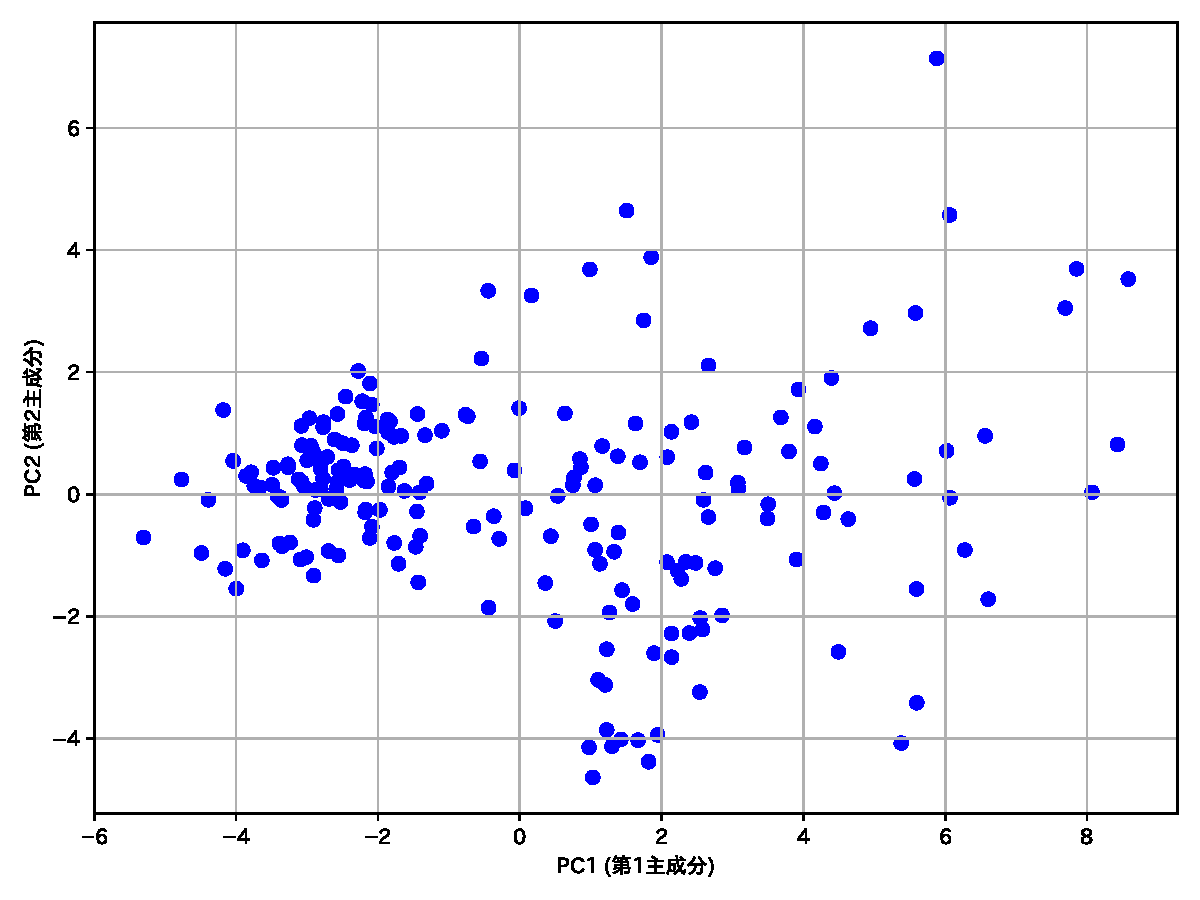
\includegraphics[width=0.7\linewidth]{Okamoto_fig/pca-10.pdf}
	\caption{ユーザのCT獲得過程パターン(10作品制作したユーザ)}
	\label{fig:pca}
 \vspace{-2mm}
\end{figure}


\subsection{(変更2-1-a)2章(改訂論文では2.2節)}
\vspace{-0.3cm}
\begin{description}
\item 修正前\\
\phantom{ }
\begin{itemize}
\item 2章タイトル:従来研究
\end{itemize}
\vspace{-0.3cm}
\item 修正後\\
\phantom{ }
\begin{itemize}
\item 2章タイトル:研究動機
\item 2.1節タイトル:従来研究
\item 2.2節タイトル:事前分析
\end{itemize}
\end{description}

\subsection{(変更2-1-b)2章(改訂論文では2.2節)}
\vspace{-0.3cm}
\begin{description}
\item 加筆後\\
\phantom{ }
Troianoら[8]\textcolor{red}{[10]}の研究では,13歳から14歳の生徒が作品制作する過程で並列,論理,同期の点数が高くなる生徒が多いが,抽象化やデータ表現の点数が高くなる生徒が少ないことを確認している.\textcolor{red}{また,同一著者らの[13]]研究では,8年生が制作したScratchゲームを用いて,ゲームジャンルがCTにどのような影響を与えるのかを調査し,アクション等の特定のゲームがCTに影響を与えることが明らかとなった.Aivalglouら[11]の研究では,Scratchプログラムの複雑さ,抽象化について調査し,プロシージャなどの抽象化の概念は一般的に使用されないことが明らかとなった.Kafaiら[12]の研究では,若者がプログラミングに取り組む上での社会的背景や文化的背景を調査している.}
\end{description}

\subsection{(変更2-1-c)2章(改訂論文では2.2節)}
\vspace{-0.3cm}
\begin{description}
\item 修正前\\
\phantom{ }
本研究では事前分析として,ユーザが初めてDeveloping以上またはMasterに到達した作品のCTスキルを調査する.表2,表3は,紙面の都合上,同じ概念を使用して制作した作品数の多いそれぞれ3パターンのみを示す.Developingに到達する作品の中で,並列,同期の点数が異なる.また,Masterに到達した作品は合計点数の分散がDevelopingに到達する作品に比べて大きく,抽象化,同期,フロー制御の点数が異なる.このように,特定の習熟度に到達した作品の中でも使用されるCTスキルが異なるため,それまでに制作した作品に使用したCTスキルも異なることが示唆される.本研究では,特定の習熟度に到達するまでの過程で使用されるCTスキル,および各CTスキルを用いた作品制作数を明らかにし,CT概念の習熟過程やCTスキルの成長パターンの理解を研究の狙いとする.
\vspace{-0.3cm}
\item 修正後\\
\phantom{ }
\color{red}
本研究では,ユーザのCTスコア獲得過程のパターンによる違いを調査するため,事前分析を行う.具体的には,従来研究\cite{Ando_2021}で用いられていたデータセットのユーザから,{$N~(3 \leq N \leq 20)$}個の作品を制作した各ユーザのCTスコア獲得過程を($N \times 7$)次元のベクトルとして平坦化し,主成分分析を行う.図\ref{fig:pca}は,11作品目にDevelopingまたはMasterの作品を制作したユーザが習熟度が向上するまでの10作品分のCT獲得過程パターンを散布図を示す.第1主成分,第2主成分の固有値はそれぞれ2.9,9.8であり1以上であるため,データを十分に説明できていると考える.その上で,散布図の全体的にばらつきが見られ,CT獲得過程のパターンがユーザによって異なることを明らかにしました.他の制作回数を持つユーザにおいても同様の傾向が見られ,CTスコア獲得過程におけるパターンの多様性を確認した.このように,ユーザによって作品の制作過程で使用されるCTスキルが異なるため,本研究では,ユーザの作品制作過程で使用されるCTスキル,および各CTスキルを用いた作品制作数を明らかにし,CT概念の習熟過程やCTスキルの成長パターンの理解を研究の狙いとする.
\color{black}
\end{description}




%--------------------------------------------------------------------------------
\newpage
\nextans
\subsection{(条件2-2)}

条件2(有用性): 
結果論になるかもしれませんが,元々CTの習熟過程,とくにCT習得順序を分析する目的だったと思いますが,調査の結果,獲得CTの共通性に注目していると拝見しました.予測でも同じCT概念を利用する確率を使っており,5章も予測する作品から遡る作品数が1つの時に予測評価値が最も高くなっているため,習熟過程とは言いがたく見えます.習熟過程というと,一般的には特定の物事に十分慣れ,自身の力として身につけていく過程全てを指しますが,本論文の分析は,特定のユーザや習熟過程の一部などに偏っていると思われます.他条件への対応で変わるかもしれませんが,現状の背景や分析方法で進める場合「習熟過程を分析するための第一歩として,同じCTスコアとなる作品を過去に作成したか(習熟過程に同様のCTスコアが存在するか)否かで,DevelopingやMasterへの到達率が変わるかを調査した」など,同じCT概念(スコア)獲得に注目したタイトル,背景,ストーリーに書き換えたが,目的と結果が一致するように感じます.習熟過程のままが適切であるとお考えの場合,その理由を回答書にてご教示ください.

\subsection{(回答2-2)}

貴重な御指摘を頂き,誠にありがとうございます.本論文では,ユーザが過去の作品の習熟順序が特定の作品(特定のCTスコアまたは特定の習熟度)の制作に影響を与えているか否かを明らかにすることを目的とし,ご指摘の通りユーザの過去の作品の「習熟過程の共通性」を分析しています.論文中でユーザ間の「習熟過程の共通性」に着目していることを加筆いたしました.ただ,ご指摘いただいた「習熟過程を分析するための第一歩として,同じCTスコアとなる作品を過去に作成したか(習熟過程に同様のCTスコアが存在するか)否かで,DevelopingやMasterへの到達率が変わるかを調査した」とは少し異なっています.「同一のユーザが同じCTスコアとなる作品を過去に作成したため特定の習熟度に到達した事例」は一部であり,多くはRQ1やRQ2で示すように,「異なるユーザが特定の習熟度に到達するまでに共通の習熟過程が存在する」ことを確認しました.具体的には,RQ1で特定の習熟度に到達するために多くのユーザが制作する作品のCTが共通していることを明らかにし,RQ2では特定の習熟度に到達する直前に制作する数作品のCTスキルが共通であった場合に,従来研究よりも高い精度での予測を実現しています.従って,大幅なストーリーの変更ではなく,論文タイトル,目的,RQ1をそれぞれ変更2-2のように加筆いたします.


\subsection{(変更2-1-c)\todo{hoge}章}
\vspace{-0.3cm}
\begin{description}
\item 加筆\\
\phantom{ }
\begin{itemize}
\item[タイトル:] Scratch ユーザのコンピュテーショナル・シンキングスキル
の習熟過程\textcolor{red}{の共通性}分析と習熟度到達予測
\item[概要: ] (省略)...本研究では,Scratch におけるユーザのコンピュテーショナル・シンキング (CT) の 習
熟過程\textcolor{red}{の共通性}を分析し...(省略)
\item[1章:] 本研究では,\textcolor{red}{習熟過程を分析するための第一歩として,}過去に制作した作品が\textcolor{red}{ユーザ間で共通する}CTスキルの\textcolor{red}{習熟過程}に基づいて,ユーザが次に制作する作品のCT習熟度が向上するか否かを予測する手法を構築する.
\item[RQ1:] CT習熟度が向上するユーザが\textcolor{red}{共通して}過去の作品で使用する CT スキルの特徴は?
\end{itemize}
\end{description}



%--------------------------------------------------------------------------------
\newpage
\nextans
\subsection{(条件2-3)}

条件3(可読性): 

2章で表2表3を参照していますが,キャプションに当たるBtoD,DtoMの説明は3章で行われています.参照するタイミングでBtoD, DtoMの説明を行ってください.同様に,表2表3で使用したデータの説明も3章で行われているものだと思われます.推敲の上,説明の順序を適切に修正してください.
また「本研究では事前分析として」とありますが,どの目的に向けた事前分析か分かりません.直前の「CT スキルの使用順は考慮していない.」に対する事前分析の目的を明示してください.

\subsection{(回答2-3)}

\todo{todo}

%貴重な御指摘を頂き,誠にありがとうございます.査読者1の方から頂いた(コメント1-1)と類する御意見と存じます.Scratchは決められた順序で学習を進めるサービスではなく,ユーザが作品制作において試行錯誤を繰り返し,コンピュテーショナル・シンキングを習熟する環境を提供しているサービスです.しかし,御指摘の通りユーザが実際に試行錯誤を繰り返してCT概念を習熟しているか否かを確認することはできず,ユーザの正確な習熟度についても明らかにすることはできません.そのため,十分に習熟しているユーザであっても,CTスコアの低い作品を制作し続ける場合,習熟度到達予測モデルでは適切に予測できないことも考えられます.


%--------------------------------------------------------------------------------
\newpage
\nextans
\subsection{(条件2-4)}

条件4(正確性): 

「作品数(重複数)を分析することで,多くのユーザが特定の習熟度に到達するまでに使用したCT概念の順番や…を明らかにすることができる」とありますが,順番は明らかになっていないのではないでしょうか?図1において,ノードA2とノードA3が入れ替わっても,重複率1.67の結果は変わらないと見受けられます.正しい表現に修正してください.

\subsection{(回答2-4)}

貴重な御指摘を頂き,誠にありがとうございます.ご指摘に通り順番は明らかになっていないため「順番」という表現を変更2-4のように削除いたします.

\subsection{(変更2-4)\todo{todo}章}
\vspace{-0.3cm}
\begin{description}
\item 修正前\\
\phantom{ }
本分析では,複数のユーザが共通のCTスキルを使用して制作した作品数(重複数)を分析することで,多くのユーザが特定の習熟度に到達するまでに使用したCT概念\textcolor{red}{\sout{の順番}}や制作した作品数などのCT概念の習熟過程を明らかにすることができる

\vspace{-0.3cm}
\item 修正後\\
\phantom{ }
本分析では,複数のユーザが共通のCTスキルを使用して制作した作品数(重複数)を分析することで,多くのユーザが特定の習熟度に到達するまでに使用したCT概念や制作した作品数などのCT概念の習熟過程を明らかにすることができる.
\end{description}



%--------------------------------------------------------------------------------
\newpage
\nextans
\subsection{(条件2-5)}

条件5(信頼性)

表4,表6において,同じ記号が続くこと(表4 作品数7,10,11〜15,18)や繰り返されること(表4 14,16,17),異なるユーザが同じパターンをたどること(表6 作品数11〜15)は面白い結果ですが,統制されていないインフォーマルラーニングにおいて,偶然このような結果が生じることは直感的ではないように感じました.調べた結果こうだったということは分かりますが,具体的な内容を示されると,より信頼性が増すと思われます.例えば,ベースが同じプログラムに対し,CT向上とは関係の無い機能(すでに獲得したCTで実装できる機能)をプロトタイピング的に実装し続けていたや,よく作成されるプログラム(入門書によく出るようなプログラム)を作成していたなど、特徴的な結果に対し実例を交えた考察を加えてください.結果に対する妥当性や信頼性が向上します.

\subsection{(回答2-5)}

貴重な御指摘を頂き,誠にありがとうございます.


\subsection{(変更2-5)\todo{todo}章}
\vspace{-0.3cm}
\begin{description}
\item 修正前\\
\phantom{ }
代表CTパスには,同じCTスキルの作品を繰り返し制作した後に習熟度が向上しているユーザを確認できる.具体的には,作品数14や16の代表CTパスは,それぞれ\texttt{\large{NBS}}や\texttt{\large{UOQV}}のCTスキルの作品を繰り返し制作して習熟度を向上している.同じCTスキルを使用している理由には,異なる種類のブロックを使用せずに,類似する作品の制作を繰り返しているためDevelopingに到達する作品を制作できずにいることが示唆される.本結果は従来研究[7]が成長に従いブロックの種類数が増加するという結果を裏付けている.また,作品数16の代表CTパスでは,CTスコアの高い作品をリミックスした作品(記号\texttt{\large{U,V,W}})を制作することで習熟度が向上していることが示唆され,従来研究[7]結果を裏付ける.

\vspace{-0.3cm}
\item 修正後\\
\phantom{ }
代表CTパスには,同じCTスキルの作品を繰り返し制作した後に習熟度が向上しているユーザを確認できる.具体的には,\textcolor{red}{作品数11や14,16の代表CTパスは,それぞれ\texttt{\large{Q}}や\texttt{\large{NBS}},\texttt{\large{UOQV}}のCTスキルの作品を繰り返し制作して習熟度を向上している.実際に繰り返し同じCTスコアを獲得しているユーザを確認したところ\footnote{https://scratch.mit.edu/projects/281002107}\footnote{https://scratch.mit.edu/projects/281003135}\footnote{https://scratch.mit.edu/projects/281004118},同じCTスコアではあるが,異なる命令処理を用いたり,プログラム構造の異なる作品を制作していることが確認した.従って,一部のBtoDユーザは自身の習得しているCT概念の作品を制作して慣れることで習熟度を向上させていることが示唆される.また,\texttt{\large{N}}のCTスキルの作品も確認したところ,紙芝居のようなアート作品が制作され,作品中で使用される画像だけ差し替えて新たに作品を制作していた.これらのユーザはリミックス等の機能を用いていないため,アート作品におけるデザインパターンが存在することが示唆された.本結果は従来研究[7]が成長に従いブロックの種類数が増加するという結果を裏付けている.}
\end{description}




%--------------------------------------------------------------------------------
\newpage
\nextans
\subsection{(条件2-6)}

条件6(妥当性): 

「また,作品数 16 の代表 CT パスでは,CT ス コアの高い作品をリミックスした作品(記号 U,V,W)を制作することで習熟度が向上していることが示唆され」とありますが,1人であることに加え他の作品数帯に同様の例がないため,本当にRemixが作用したか分からず,裏付けとまでは言えないように感じます.先行研究でも同じように数回のRemixとオリジナル作品の作成を繰り返し,オリジナル作品の点数が1点上がっていたのでしょうか?それとも1回のRemixの前後でスコアが向上するのでしょうか?Remixに関する調査は本研究の対象外だと思いますが,人数が1名であることと,先行研究の内容を踏まえ,適切な表記に修正してください.

\subsection{(回答2-6)}

貴重な御指摘を頂き,誠にありがとうございます.御指摘の通り,習熟度が向上している理由として十分なデータに基づき分析結果を示せているとは言い難いため,ご指摘いただいた文章は削除いたします.当該文章を削除したとしても知見2の主張が変わるようなことはございません.

リミックスに関する従来研究では,Scratchのシステムを構築した開発者は,Jenkins [参考1] を引用してコンテンツへの能動的関与の理想的なモデルであると主張し次のように述べている.「Scratchは,ユーザ同士の交流によってScratch 作品のオリジナルの構成要素を共有したり、適切なものにしたりできる」[参考2] と説明し,Scratchのユーザーは他ユーザの作品のリミックスを通じて学習できると述べている.ただし,リミックスを支援・促進する方法、ユーザーによるリミックスの受容,リミックス作品の品質に関する理論は研究されているが,リミックスが学習への経路として正しく機能しているかは十分に研究されていません.ユーザに学習への経路を与える有用なリミックス作品を提供することで,リミックスを通じた学習が可能になるのかは本研究でも今後の課題とさせていただきます.

\noindent[参考1] H. Jenkins, Convergence Culture: Where Old and New Media Collide, New York: New York University Press, 2008.\\
\noindent[参考2] A. Monroy-Hern\'{a}ndez, ScratchR: Sharing user-generated programmable media,
In Proceedings of the 6th International Conference on Interaction Design and Children, p.167‒ 168, IDC'07, Association for Computing Machinery, 2007.



%--------------------------------------------------------------------------------
\newpage
\nextans
\subsection{(条件2-7)}

条件7(新規性): 

知見1の結論は先行研究を交えて議論を行ってください.本研究で得られた知見と,[8]などの先行研究で得られている知見の区別が付かず,新規性が評価できません.加えて,ページ数の問題があることは分かりますが,表4や表6の各作品数のユーザ数は少なく,一般性が評価できません.本調査で作品制作の多様性を調査するのではなく,共通性を調べるのであれば,DevelopingやMasterに到達したときの点数分布(各CTの習熟)が同じユーザ同士で比較しなくても良いのではないでしょうか?DevelopingやMasterに到達したときの点数分布が同じユーザで比較する場合,その理由を述べてください.5章の予測モデルにて精度が向上しているため,得られた結果の一部の一般性は評価できるのかもしれませんが,今回得られた各知見が,表2,表3の順位2位,3位などでも同じであるかを調査するなどして,各結論の妥当性や一般性を明示してください.

\subsection{(回答2-7)}

貴重な御指摘を頂き,誠にありがとうございます.従来研究では作品制作を重ねていく過程で,個々の作品のCTスキルの変遷を確認していないため,知見1の成果は従来研究では明らかにされていない,本研究が初めて明らかにした成果となります.また,本研究でDevelopingやMasterにそれぞれ到達したときの点数分布が同じユーザで比較している理由は2点あります.1つ目の理由は本論文の動機づけとなった先行研究[9]と同じ分析方法をとっているからです.2つ目はRQ1はRQ2の動機づけとなっており,RQ2でDevelopingやMasterにそれぞれ到達したときの点数分布が同じユーザで比較しているからです.ご指摘の通り,表2,表3(改訂論文における表4,表5)の順位1位だけでは本結論の妥当性を十分に主張できていないと考え,\todo{順位2位,3位に関しても調査いたしました.この結果は回答書のみに書けると...良いが...}


%貴重な御指摘を頂き,誠にありがとうございます.査読者1の方から頂いた(コメント1-1)と類する御意見と存じます.Scratchは決められた順序で学習を進めるサービスではなく,ユーザが作品制作において試行錯誤を繰り返し,コンピュテーショナル・シンキングを習熟する環境を提供しているサービスです.しかし,御指摘の通りユーザが実際に試行錯誤を繰り返してCT概念を習熟しているか否かを確認することはできず,ユーザの正確な習熟度についても明らかにすることはできません.そのため,十分に習熟しているユーザであっても,CTスコアの低い作品を制作し続ける場合,習熟度到達予測モデルでは適切に予測できないことも考えられます.






\subsection{(変更2-7-a)4.1節}
\vspace{-0.3cm}
\begin{description}
\item 修正前\\
\phantom{ }
本研究では,ユーザがDeveloping以上の作品,またはMasterの作品を制作するために,過去に制作した作品で使用したCTスコアの系列(CT パス)を追跡する.
\vspace{-0.3cm}
\item 修正後\\
\phantom{ }
\textcolor{red}{
従来研究[9]において,BtoDユーザとDtoMユーザ間で習熟度が向上するまでに制作する作品のCT概念の特徴は異なることが明らかとなった.そのため,本研究では,BtoDユーザ,DtoMユーザそれぞれで習熟度が向上するまでに制作した作品で使用したCTスコアの系列(CTパス)を追跡する.
}
\end{description}

\subsection{(変更2-7-b)4.3節}
\vspace{-0.3cm}
\begin{description}
\item 加筆後\\
\phantom{ }
\textcolor{red}{[変更2-7-b]また,RQ1における各知見の一般性を評価するため,表3,表7の上位2位についても同様の分析を実施した.結果として知見1〜知見3と同様の特徴が見られたことから,RQ1の結果は妥当であるといえる.しかし,知見2で繰り返し制作される作品のCTスコアが異なることや,知見3で見られた記号\texttt{\large{M,c,d,Q,f,g,O}}(表6の青文字))のようなCTスコアのパターンは見られなかったことから,ユーザが習熟度向上時に制作した作品のCTスコアによって作品制作過程で獲得するCTスコアは異なるが,BtoDユーザ,DtoMユーザともにCT獲得過程の特徴は類似していることが明らかとなった.}
\end{description}




%--------------------------------------------------------------------------------
\newpage
\nextans
\subsection{(条件2-8)}

条件8(可読性,妥当性):

条件7と関係しますが,今回の調査では代表CTパスではなかったユーザがほとんどだと拝見します.そのため,知見1と知見2 の妥当性が評価できません.また,最も多いCTパス(代表CTパス)であるのに,複数の項目にて,ユーザ数が1であることも分かりません.例えば表4の作品数2においてBBが最も多いCTパスであり,その人数は42名中18名だったという結論は分かりますが,作品数11にて,NNNNNNNNPBIが最も多いCTパスであり,その人数は3名中1名だったとなると,最も多いとは言えないのではないでしょうか(全員ばらばらのCTパスで表通性はなかったのではないでしょうか).表4・表6の解釈が分からず,また知見1.知見2の根拠も不明瞭になっています.代表CTパスについて1名時の説明を加え,知見では人数も考慮した考察,結果を示してください.

\subsection{(回答2-8)}

%貴重な御指摘を頂き,誠にありがとうございます.査読者1の方から頂いた(コメント1-1)と類する御意見と存じます.Scratchは決められた順序で学習を進めるサービスではなく,ユーザが作品制作において試行錯誤を繰り返し,コンピュテーショナル・シンキングを習熟する環境を提供しているサービスです.しかし,御指摘の通りユーザが実際に試行錯誤を繰り返してCT概念を習熟しているか否かを確認することはできず,ユーザの正確な習熟度についても明らかにすることはできません.そのため,十分に習熟しているユーザであっても,CTスコアの低い作品を制作し続ける場合,習熟度到達予測モデルでは適切に予測できないことも考えられます.

%--------------------------------------------------------------------------------
\newpage
\nextans
\subsection{(条件2-9)}

条件9(正確性): 

「本予測手法では,従来研究における CT スキルの使用 順に着目しない手法による誤った予測を回避するために, ユーザ間の CT パスの共通性に基づいて特定の習熟度に到 達する予測可能なユーザを明らかにする.…ただし,本手法 は予測対象となるユーザが過去に制作した作品の CT パス と一致した場合に予測できるが,過去に制作した作品の中 に同一の CT パスを有する作品が存在しなければ予測でき ない.」
ユーザ間のCTパスから分かる情報と,ユーザが過去に制作した作品の CT パスが混合しており,意味がとれませんでした.なぜユーザ間の CT パスの共通性に基づくと,従来研究における 「CT スキルの使用 順に着目しない手法による誤った予測を回避することができる」のかを明示してください.すでに本文に書かれている場合,その旨回答書にてご指摘下さい.また,CTパスは過去に作成したCTスコアの系列と書かれています.ユーザが過去に制作した作品の CT パスとは何でしょうか?例えば表5で言う,ABCFで作品を作ったユーザは予測できず,ABCABCの作品を作ったユーザは予測できるということでしょうか?ABCAも予測できるのでしょうか?表5のCT表を利用するなどして,例を使い本文にて修正・補足してください.表12で実例がありますが,結果の説明の際に簡単な例を用いて説明されたがわかりやすいです.現状は表12を見るまで結果のイメージが持てません.

\subsection{(回答2-9)}

%貴重な御指摘を頂き,誠にありがとうございます.査読者1の方から頂いた(コメント1-1)と類する御意見と存じます.Scratchは決められた順序で学習を進めるサービスではなく,ユーザが作品制作において試行錯誤を繰り返し,コンピュテーショナル・シンキングを習熟する環境を提供しているサービスです.しかし,御指摘の通りユーザが実際に試行錯誤を繰り返してCT概念を習熟しているか否かを確認することはできず,ユーザの正確な習熟度についても明らかにすることはできません.そのため,十分に習熟しているユーザであっても,CTスコアの低い作品を制作し続ける場合,習熟度到達予測モデルでは適切に予測できないことも考えられます.

%--------------------------------------------------------------------------------
\newpage
\nextans
\subsection{(条件2-10)}

条件10:(有用性) 

「Masterに到達するユーザと到達しないユーザは直前に制作する作品で,共通のCT概念を使用する作品を制作していることが示唆される」例えば5作品目でMasterに到達する場合,4作品目も5作品目と同様のCTを獲得する作品を作っているということでしょうか?その場合,Masterに到達しないユーザの「直前の作品」は何を指すのでしょうか?文章の意味を取ることが難しいため,補足をお願いします.

\subsection{(回答2-10)}
貴重な御指摘を頂き,誠にありがとうございます.「直前の作品」という曖昧な表現となっていた点につきまして,謹んでお詫び申し上げます.本研究において「直前の作品」とは特定の習熟度(DevelopingやMaster)の作品を制作する\todo{一つ前の作品}を指します.\todo{20作品の件...どうしよ...}


%貴重な御指摘を頂き,誠にありがとうございます.査読者1の方から頂いた(コメント1-1)と類する御意見と存じます.Scratchは決められた順序で学習を進めるサービスではなく,ユーザが作品制作において試行錯誤を繰り返し,コンピュテーショナル・シンキングを習熟する環境を提供しているサービスです.しかし,御指摘の通りユーザが実際に試行錯誤を繰り返してCT概念を習熟しているか否かを確認することはできず,ユーザの正確な習熟度についても明らかにすることはできません.そのため,十分に習熟しているユーザであっても,CTスコアの低い作品を制作し続ける場合,習熟度到達予測モデルでは適切に予測できないことも考えられます.


\subsection{(変更2-10-a) 5.2.1項}
\vspace{-0.3cm}
\begin{description}
\item 修正前\\
\phantom{ }
したがって,Developingに到達する直前に制作する作品で,共通のCT概念を使用する作品を制作していることが示唆される.
\vspace{-0.3cm}
\item 修正後\\
\phantom{ }
\textcolor{red}{\UnderlineTex{したがって,Deveolopingに到達するユーザがDeveolopingの作品を制作する直前に共通のCT概念を使用する作品を制作していることが示唆される.また,同様にDeveolopingに到達しないユーザも20作品目の直前に制作する作品で共通のCT概念を使用する作品を制作していることが示唆される.}}
\end{description}


\subsection{(変更2-10-b) 5.2.1項}
\vspace{-0.3cm}
\begin{description}
\item 修正前\\
\phantom{ }
したがって,Master に到達するユーザと到達しないユーザは直前に制作する作品で,共通のCT 概念を使用する作品を制作していることが示唆される.
\vspace{-0.3cm}
\item 修正後\\
\phantom{ }
\textcolor{red}{\UnderlineTex{したがって,Masterに到達するユーザがMasterの直前に制作する作品で共通のCT概念を使用する作品を制作していることが示唆される.また,同様にMasterに到達しないユーザも20作品目の直前に制作する作品で共通のCT概念を使用する作品を制作していることが示唆される.}}
\end{description}






%--------------------------------------------------------------------------------
\newpage
\nextans
\subsection{(条件2-11)}

条件11(正確性,可読性): 

「RQ2 において,BtoD ユーザが Developing に到達する直前の CT パスは非 BtoD ユーザよりも重複数が多い事が 明らかになった.」これは図6を指しているのでしょうか.その場合,図6はBtoD ユーザが *Developing に到達する直前の CT パス*かどうかは書かれていないように見受けられます.どこを読み取れば良いか明示してください.
また,以降の文章は全て繋がりが分かりません.なぜ急にMasterが出てくるのか,なぜ以降の分析ではモデルを用いないのにモデルに学習させるパスの長さの話がでたのか,なぜBtoD ユーザのみを対象に 2 作品目または 3 作品目に Developing に到達する作品を分析したのか,それぞれの理由を詳述してください.追記の必要が無い場合,回答書でご説明ください.

\subsection{(回答2-11)}

%貴重な御指摘を頂き,誠にありがとうございます.査読者1の方から頂いた(コメント1-1)と類する御意見と存じます.Scratchは決められた順序で学習を進めるサービスではなく,ユーザが作品制作において試行錯誤を繰り返し,コンピュテーショナル・シンキングを習熟する環境を提供しているサービスです.しかし,御指摘の通りユーザが実際に試行錯誤を繰り返してCT概念を習熟しているか否かを確認することはできず,ユーザの正確な習熟度についても明らかにすることはできません.そのため,十分に習熟しているユーザであっても,CTスコアの低い作品を制作し続ける場合,習熟度到達予測モデルでは適切に予測できないことも考えられます.

%--------------------------------------------------------------------------------
\newpage
\nextans
\subsection{(条件2-12)}

条件12(正確性,可読性): 

6.2における,パス重複数が18でパターン1とは,2名が18回(=Developingに到達して以降全ての作品で)同じCTパスをたどり,他にパス重複数が18のユーザはいなかったと言うことでしょうか.パターンとは何を示すのでしょうか.いずれの場合も,BtoDとDtoMを直接比較しない理由は何でしょうか.また,最大パス重複数を見る場合,最大のもの(18回も同じCTパスをたどるもの)が少ないことは当たり前に思います.重複率や散布図などを使わない理由はなぜでしょうか.1〜2or3回目までのプログラムと,2or3〜20回目のプログラムを比較するなら,対象プログラムの母数も大きく異なります.条件11の指摘の通り,なぜ2,3作品目で調査したかも分かりませんため,RQ3の結論は解釈できません.
「CT スキルの使用履歴の違いによって特定の習熟度に到達した 作品の CT スコアの偏りを分析」とありますが,本目的に分析手法が従っていないように見えます.文章を全体的に推敲し,目的とアプローチが一致するようにしてください.

\subsection{(回答2-12)}

%貴重な御指摘を頂き,誠にありがとうございます.査読者1の方から頂いた(コメント1-1)と類する御意見と存じます.Scratchは決められた順序で学習を進めるサービスではなく,ユーザが作品制作において試行錯誤を繰り返し,コンピュテーショナル・シンキングを習熟する環境を提供しているサービスです.しかし,御指摘の通りユーザが実際に試行錯誤を繰り返してCT概念を習熟しているか否かを確認することはできず,ユーザの正確な習熟度についても明らかにすることはできません.そのため,十分に習熟しているユーザであっても,CTスコアの低い作品を制作し続ける場合,習熟度到達予測モデルでは適切に予測できないことも考えられます.

%--------------------------------------------------------------------------------
\newpage
\nextans
\subsection{(参考意見2-1)}

・条件でも指摘していますが,全体的に「示唆される」の根拠となる説明が粗く,主観や一部の結果を拡大解釈しているように感じます.また論理の文であるため「示唆される」の表現自体多様は避け,結果のどの部分から何が客観的に分かるかを明示するのが望ましいです.可能な限り,結果を示せるように分析・結果をまとめてください.

\subsection{(参考意見への回答2-1)}

貴重な御指摘を頂き,誠にありがとうございます.論文中に「示唆される」という文言を多様し,本論文の主張を正しく表現できていない説明が散見していました.謹んでお詫び申し上げます.つきまして,論文中の表現を今一度見直し,一部「示唆される」を削除する,または表現を変えました.再査読いただく際の可読性が下がることを懸念し,変更箇所を個別にラベル付与しておりません.ご了承ください.



%--------------------------------------------------------------------------------
\newpage
\nextans
\subsection{(参考意見2-2)}

・表14はどちらが2作品目でどちらが3作品目のデータか明示した方がわかりやすいです.

\subsection{(参考意見への回答2-2)}

貴重な御指摘を頂き,誠にありがとうございます.査読者1の方から頂いた(条件1-2-7)と類する御意見と存じます.ご指摘の通り,表中に「2作品目」「3作品目」の記入漏れがありました.謹んでお詫び申し上げます.論文修正にともない表番号が変わったため,表14は変更C2-2のように加筆いたしました.

\subsection{(変更C2-2)表14(論文改訂後,表16)}
\vspace{-0.3cm}
\begin{description}
\item 修正前\\
\phantom{ }
\renewcommand{\thetable}{\arabic{table}}
\setcounter{table}{13}
\begin{table}[h]
  \caption{2作品目または3作品目にDevelopingの作品を制作したユーザのCTパス重複数とそのパターン数}
  \label{tab:goal-pattern-2}
  %\vspace{2mm}
  \centering
  \scalebox{0.87}{
  \begin{tabular}{c|c|ccc|c|c}
    \cline{1-3}\cline{5-7}
    順位 & パス重複数 & パターン数 && 順位 & パス重複数 & パターン数\\
    \cline{1-3}\cline{5-7}
    1 & 18 & 1 &&1 & 5 & 2\\
    \cline{1-3}\cline{5-7}
    2 & 11 & 1 &&2 & 4 & 2\\
    \cline{1-3}\cline{5-7}
    3 & 9 & 1 &&3 & 3 & 2\\
    \cline{1-3}\cline{5-7}
    4 & 8 & 1 &&4 & 2 & 10\\
    \cline{1-3}\cline{5-7}
    % 5 & 7 & 3\\
    % \hline
  \end{tabular}
    }
   \vspace{-2mm}
\end{table}
\vspace{-0.3cm}
\item 修正後\\
\phantom{ }
\renewcommand{\thetable}{\arabic{table}}
\setcounter{table}{15}
\begin{table}[h]
  \caption{2作品目または3作品目にDevelopingの作品を制作したユーザのCTパス重複数とそのパターン数}
  \label{tab:goal-pattern-2}
  \centering
  \scalebox{0.87}{
  \begin{tabular}{c|c|c||c|c|c}
    \cline{1-3}\cline{4-6}
    \multicolumn{3}{c||}{\textcolor{red}{\UnderlineTex{2作品目}}} & \multicolumn{3}{c}{\textcolor{red}{\UnderlineTex{3作品目}}} \\
    \cline{1-3}\cline{4-6}
    順位 & パス重複数 & パターン数 & 順位 & パス重複数 & パターン数 \\
    \cline{1-3}\cline{4-6}
    1 & 18 & 1 & 1 & 5 & 2 \\
    \cline{1-3}\cline{4-6}
    2 & 11 & 1 & 2 & 4 & 2 \\
    \cline{1-3}\cline{4-6}
    3 & 9 & 1 & 3 & 3 & 2 \\
    \cline{1-3}\cline{4-6}
    4 & 8 & 1 & 4 & 2 & 10 \\
    \cline{1-3}\cline{4-6}
  \end{tabular}
  }
   \vspace{-2mm}
\end{table}

\end{description}

%--------------------------------------------------------------------------------
\newpage
\nextans
\subsection{(参考意見2-3)}

・以下は誤字だと思われます.
「特に,CTスコアを3つの区分(CT習熟度)に分類し,0点から7点をBasic」→0点の前が半角です

「表8は従来BtoDモデルと提案BtoDモデル (L=1) の予測結果を示す.従来手法に比べて高い精度で予測することができた.(7ページ目右下)」→表9のDtoMの話だと思います.

「表 13 から,2 作品目または 3 作品目 で Developing に到達した」→表14"

\subsection{(参考意見への回答2-3)}

貴重な御指摘を頂き,誠にありがとうございます.ご指摘の通りの誤字がありました.謹んでお詫び申し上げます.それぞれ論文中で[変更C2-3]のラベルを付して,変更いたしました.

	
%--------------------------------------------------------------------------------


\end{document}
